\PassOptionsToPackage{usenames,dvipsnames}{xcolor}

\documentclass[20pt, a0paper, landscape, margin=0mm, innermargin=15mm, blockverticalspace=15mm, colspace=15mm, subcolspace=8mm]{tikzposter}
\usepackage[T1]{fontenc}
\usepackage[utf8]{inputenc}
\usepackage[english]{babel}

\usepackage{amsmath,amsfonts,amssymb,mathtools}

%\usepackage[usenames,dvipsnames]{xcolor}
\usepackage{graphicx,mwe}
\usepackage{filecontents}% http://ctan.org/pkg/filecontents
\usepackage{tikz}
\usepackage{multicol}
\usepackage{adjustbox}
\usepackage{authblk}

\usepackage{enumitem}

\usepackage{caption}
\captionsetup{font=large}

\usepackage{url}
\usepackage[colorlinks=false]{hyperref}
\urlstyle{tt}


%\newcommand*{\doi}[1]{\href{https://doi.org/#1}{\nolinkurl{https://doi.org/#1}}}
\newcommand*{\doi}[1]{\href{https://doi.org/#1}{\nolinkurl{doi:#1}}}


% university colors based on branding guides
\definecolor{OSUorange}{HTML}{C34500}
\definecolor{UConnBlue}{HTML}{000E2F}
\definecolor{GoogleBlue}{HTML}{0266C8}

% \makeatletter
% \def\TP@titlegraphictotitledistance{-4cm}
% \settitle{ \centering \vbox{
% \@titlegraphic \\ [\TP@titlegraphictotitledistance]
% \centering
% \color{titlefgcolor} {\bfseries \Huge \@title \par} % add \sc for smallcaps
% \vspace*{2em}
% {\huge \@author \par} \vspace*{1em} {\LARGE \@institute}
% }}
% \makeatother

%% Code for increasing tikzfigure caption font size
% \renewenvironment{tikzfigure}[1][]{
%   \def \rememberparameter{#1}
%   \vspace{10pt}
%   \refstepcounter{figurecounter}
%   \centering
%   }{
%     \ifx\rememberparameter\@empty
%     \else %nothing
%     \\[10pt]
%     {\large Fig.~\thefigurecounter: \rememberparameter}
%     \fi
% }


%% Set up a logo on each side
\makeatletter
\newcommand\insertlogoi[2][]{\def\@insertlogoi{\includegraphics[#1]{#2}}}
\newcommand\insertlogoii[2][]{\def\@insertlogoii{\includegraphics[#1]{#2}}}
\newlength\LogoSep
\setlength\LogoSep{-2cm}

% \insertlogoi[width=18cm]{OSU-color-horz}
% \insertlogoii[width=18cm]{UConn-color-horz}

\def\TP@titlegraphictotitledistance{-4cm}
\settitle{ \centering \vbox{
%\@titlegraphic \\ [\TP@titlegraphictotitledistance]
\centering
\color{titlefgcolor} {\bfseries \Huge \@title \par} % add \sc for smallcaps
\vspace*{2em}
{\huge \@author \par} \vspace*{1em} {\LARGE \@institute}
}}

\renewcommand\maketitle[1][]{  % #1 keys
    \normalsize
    \setkeys{title}{#1}
    % Title dummy to get title height
    \node[transparent,inner sep=\TP@titleinnersep, line width=\TP@titlelinewidth, anchor=north, minimum width=\TP@visibletextwidth-2\TP@titleinnersep]
        (TP@title) at ($(0, 0.5\textheight-\TP@titletotopverticalspace)$) {\parbox{\TP@titlewidth-2\TP@titleinnersep}{\TP@maketitle}};
    \draw let \p1 = ($(TP@title.north)-(TP@title.south)$) in node {
        \setlength{\TP@titleheight}{\y1}
        \setlength{\titleheight}{\y1}
        \global\TP@titleheight=\TP@titleheight
        \global\titleheight=\titleheight
    };

    % Compute title position
    \setlength{\titleposleft}{-0.5\titlewidth}
    \setlength{\titleposright}{\titleposleft+\titlewidth}
    \setlength{\titlepostop}{0.5\textheight-\TP@titletotopverticalspace}
    \setlength{\titleposbottom}{\titlepostop-\titleheight}

    % Title style (background)
    \TP@titlestyle

    % Title node
    \node[inner sep=\TP@titleinnersep, line width=\TP@titlelinewidth, anchor=north, minimum width=\TP@visibletextwidth-2\TP@titleinnersep]
        at (0,0.5\textheight-\TP@titletotopverticalspace)
        (title)
        {\parbox{\TP@titlewidth-2\TP@titleinnersep}{\TP@maketitle}};

    % \node[inner sep=0pt,anchor=west]
    %   at ([xshift=-\LogoSep]title.west)
    %   {\@insertlogoi};
    %
    % \node[inner sep=0pt,anchor=east]
    %   at ([xshift=\LogoSep]title.east)
    %   {\@insertlogoii};

    % Settings for blocks
    \normalsize
    \setlength{\TP@blocktop}{\titleposbottom-\TP@titletoblockverticalspace}
}
\makeatother

\setlength{\columnsep}{2cm}


\title{\parbox{0.7\linewidth}{\centering The Journal of Open Source Software}}

\author[1]{Arfon M.\ Smith}
\author[2]{Lorena A.\ Barba}
\author[3]{George Githinji}
\author[4]{Melissa Gymrek}
\author[5]{Kathryn Huff}
\author[6]{Daniel S.\ Katz}
\author[7]{Christopher R.\ Madan}
\author[8]{Abigail Cabunoc Mayes}
\author[9]{Kevin M.\ Moerman}
\author[10]{Kyle E.\ Niemeyer}
\author[11]{Pjotr Prins}
\author[12]{Karthik Ram}
\author[13]{Ariel Rokem}
\author[14]{Tracy K.\ Teal}
\author[15]{Jake Vanderplas}

\affil[1--15]{\textit{Affiliations listed below}}

\institute{\url{http://joss.theoj.org/}}

\date{}



\usetitlestyle{Filled}

\begin{document}

\maketitle

\begin{columns} % See Section 4.4
    \column{0.25} % See Section 4.4
    \block{JOSS: Journal of Open Source Software}{

    \begin{tikzfigure}
    
\includegraphics[width=0.95\linewidth]{JOSS-logo.png}
    \end{tikzfigure}

    \vspace{1.5em}

    {\Large
    The Journal of Open Source Software (JOSS) is a developer-friendly journal
    for research software packages.
    }

    \vspace{2em}

    Requirements for submission:
    \begin{itemize}
        \item Your software should be open source as per \href{https://opensource.org/osd}{the OSI definition}
        \item Your software should have a research application (i.e., be research software)
        \item You should be a major contributor to the software you are submitting
        \item Your software should be a significant contribution to the available open-source software that
        either enables some new research challenges to be addressed or makes addressing
        research challenges significantly better (e.g., faster, easier, simpler)
        \item Your software should be feature complete---no half-baked solutions
    \end{itemize}

    } % end block

    \column{0.5}
    \block{Publication process}{

    % {\large If you've already licensed your code and have good documentation
    % then we expect that it should take \textbf{less than an hour} to prepare and
    % submit your paper to JOSS.}

    \begin{tikzfigure}
    
\includegraphics[width=0.75\linewidth]{JOSS-statement}
    \end{tikzfigure}

    \begin{tikzfigure}
    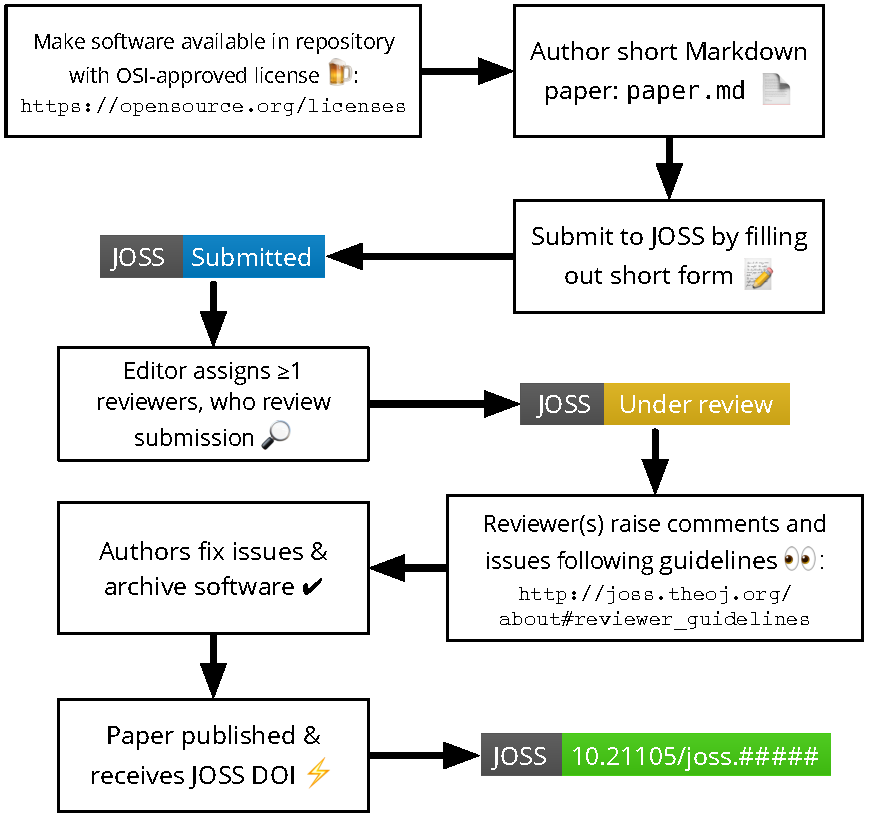
\includegraphics[width=0.58\linewidth]{JOSS-flowchart}
    \end{tikzfigure}

    }

    \column{0.25}
    \block{Paper statistics}{
    %
    \begin{tikzfigure}
    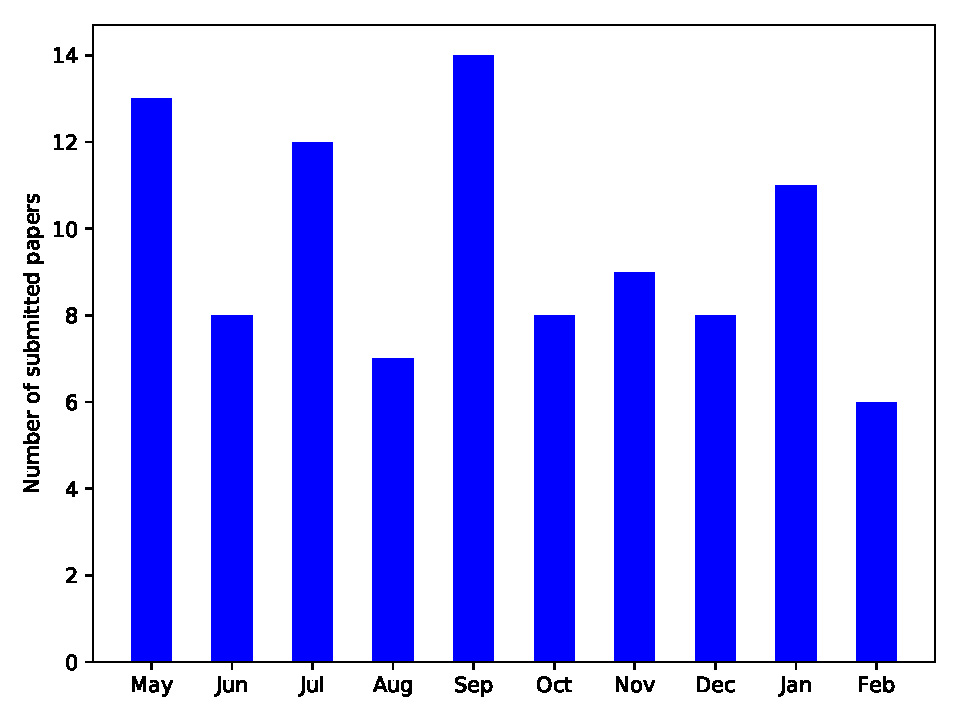
\includegraphics[width=0.95\linewidth]{JOSS-submitted-papers}
    \end{tikzfigure}
    \captionof*{figure}{Number of papers \textbf{submitted} since JOSS's creation.
    Papers currently under review: 31}
    %
    \begin{tikzfigure}
    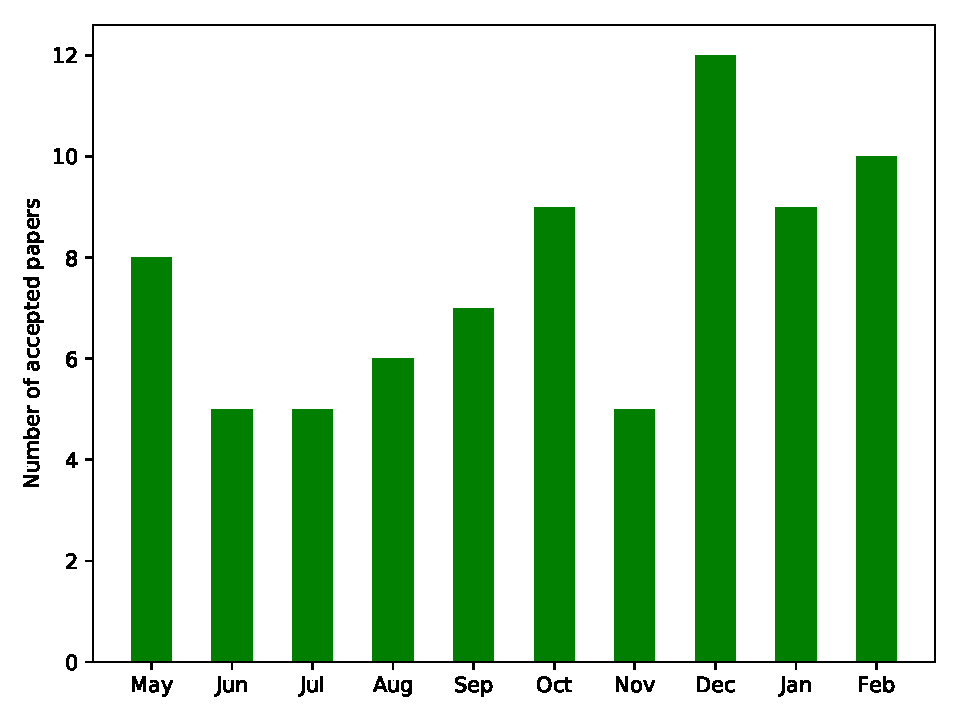
\includegraphics[width=0.95\linewidth]{JOSS-accepted-papers}
    \end{tikzfigure}
    \captionof*{figure}{Number of papers \textbf{accepted} since JOSS's creation.
    Total papers published: 76}
    %
    } % end block
    %
\end{columns}

% bottom
\begin{columns}
    \column{0.25}
    \block{Business model}{

    JOSS is an open-access journal \textbf{committed to running
    at minimal costs, with zero publication fees (article processing charges) or subscription
    fees}. With volunteer effort from our editorial board, community reviewers, donations, and
    minimal infrastructure costs we believe JOSS can remain a free community service.

    \vspace{0.5em}

    Operating costs:
    \begin{itemize}[leftmargin=1cm,topsep=0pt,noitemsep]
        \item Annual \href{http://www.crossref.org/02publishers/20pub_fees.html}{Crossref membership}: \$275 / year
        \item JOSS paper DOIs: \$1 / accepted paper
        \item JOSS website hosting (Heroku): \$19 / month
    \end{itemize}

    \vspace{0.5em}

    \textbf{Cost per paper:} \$3.50 (assuming 200 papers per year)

    } % end block

    \column{0.5}
    \block{Editorial board affiliations}{
    \begin{multicols}{2}
    {
    \begin{enumerate}[leftmargin=1cm,topsep=0pt,noitemsep]
        \item Data Science Mission Office, Space Telescope Science Institute
        \item Mechanical and Aerospace Engineering, George Washington University
        \item KEMRI--Wellcome Trust Research Programme
        \item Departments of Computer Science and Engineering \& Medicine, University of California, San Diego
        \item Department of Nuclear, Plasma, and Radiological Engineering, University of Illinois at Urbana--Champaign
        \item NCSA, CS, ECE, iSchool, University of Illinois at Urbana--Champaign
        \item Department of Psychology, Boston College
        \item Mozilla Foundation
        \item MIT Media Lab
        \item School of Mechanical, Industrial, and Manufacturing Engineering, Oregon State University
        \item Health Science Center, University of Tennessee, \& University Medical Centre Utrecht
        \item Institute for Data Science, University of California, Berkeley
        \item eScience Institute, University of Washington
        \item Data Carpentry \& Michigan State University
        \item eScience Institute, University of Washington
    \end{enumerate}
    }
    \end{multicols}
    }

    \column{0.25}
    \block{Further information}{

    {\colorlet{innerblocktitlebgcolor}{GoogleBlue}
    \colorlet{innerblocktitlefgcolor}{white}
    \innerblock{Journal home}{\centering{\url{http://joss.theoj.org/}}}
    \innerblock{Location of reviews}{\centering{\url{https://github.com/openjournals/joss-reviews}}}
    %\innerblock{JOSS source code}{\centering{\url{https://github.com/openjournals/joss}}}
    }
    %
    \vspace{1em}
    %
    \begin{minipage}{0.4\linewidth}
    \begin{tikzfigure}
    
\includegraphics[width=\linewidth]{cc-by}
    \end{tikzfigure}
    \end{minipage}
    \hfill
    \begin{minipage}{0.55\linewidth}
    This work is licensed under a Creative Commons Attribution 4.0 International License:
    \url{http://creativecommons.org/licenses/by/4.0/}.
    \end{minipage}

    } % end further information block

\end{columns}


\end{document}
